\section{RQ3: Can Deletion Be Audited?}\label{sec:rq3}

An auditor receives a model and must decide whether it behaves as
if it had trained on the deleted era. The audit of
Section~\ref{sec:method} compares two populations of ten seeds
each, references trained with the era and oracles retrained without
it, on their fit to the deleted windows. The separation $d'$ is the
standardized distance between the two populations. Near zero, the
populations overlap, and deletion cannot be certified from
behaviour. We ask whether the audit succeeds at the level of an
era, whether it succeeds at the level of a single training window,
and what treating overlapping windows as independent does to its
confidence.

\begin{figure}[t]
\centering
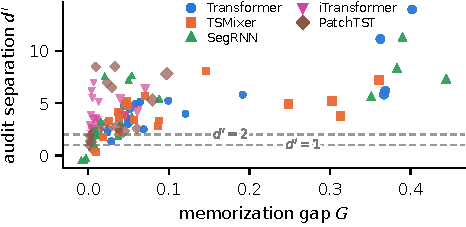
\includegraphics[width=0.92\columnwidth]{figs/fig_audit}
\caption{Audit separation $d'$ against the memorization gap $G$
for all 100 cells of architecture, deleted year, and fold (\Lone).
Crisis-year points are drawn larger, and the dashed lines mark
$d' = 1$ and $d' = 2$. All five architectures appear: an auditor
cannot presume the audited model is deployable, and the unverifiable
cells concentrate among the weak absorbers.}
\label{fig:audit}
\end{figure}

\subsection{Era-level auditing}

Figure~\ref{fig:audit} reports the audit in all 100 cells of
architecture, deleted year, and fold, instantiating the population
auditor of membership inference~\cite{carlini2022lira}. Each point
places one cell by its memorization gap from Section~\ref{sec:rq1}
on the horizontal axis and its audit separation on the vertical
axis. The figure therefore asks whether what a model memorized
decides what an auditor can see.

Across the grid the separation spans $-0.4$ to $14.0$. Removing the
crisis year from a heavy memorizer separates the two populations
completely. Removing a low- to medium-volatility year from a weak
memorizer leaves them indistinguishable from chance. What decides
the outcome is memorization. Separation rises with the gap across
the grid, and every cell the auditor cannot resolve is one where
the model had memorized almost nothing. Seventeen per cent of the
cells fall below $d' = 2$.

A legitimate deletion can therefore be unverifiable. The model did
not keep the data. It never memorized enough of it for the absence
to leave a trace. Auditability is a property of what was learned,
not of what was deleted, and a null audit is not evidence of
compliance.

\subsection{Window-level auditing}

A record-level right to erasure would require the audit to work on
a single training window. We therefore score each window separately
and ask how often the reference fits a window better than its own
oracle. The chance level of this win rate is one half. The win rate
stays near chance everywhere. Its median is just above one half,
and the best cell in the grid reaches only $0.69$. The win rate
rises with memorization, as the era-level separation does, but
never far enough to certify anything about a single window.
Whatever granularity a data contract names, it cannot be the
GDPR-style single record~\cite{gdpr2016}.

\subsection{Overlapping windows and audit power}

The window counts overstate the audit's evidence unless their
dependence is respected. Each forget day contributes about 480
windows, one per stock, and within a day those windows share one
market cross-section. The day mean therefore carries almost all of
the information, and the effective sample is the days, not the
windows. Treating windows as independent records inflates the audit
statistic by a median factor of $1.9$ across the grid, before any
window-level multiplicity is counted. HAC standard errors on panel
audit statistics are mandatory, not cosmetic.

Two further facts bound what an audit can promise. Extra forget
data does not buy power past the dispersion of the gap across
retraining seeds, which no amount of data lowers. And the minimum
detectable gap of the daily audit statistic, derived in the
released protocol, should accompany any audit verdict.
